\documentclass[12pt, a4paper, one side]{article}
\usepackage[utf8]{inputenc}
\usepackage[french]{babel}
\usepackage{biblatex}
\usepackage{listings}
\usepackage{xcolor}
\usepackage{hyperref}
\usepackage{graphicx}
\usepackage{minted}

\bibliography{reference}

\usepackage{comment}

\lstset{
    basicstyle=\itshape,
    xleftmargin=3em,
    literate={->}{$\rightarrow$}{2}
        {^}{$\uparrow$}{1}
        {↓}{$\downarrow$}{1},
    morekeywords={method_body},
    basicstyle=\small
}

\definecolor{codegreen}{rgb}{0,0.6,0}
\definecolor{codegray}{rgb}{0.5,0.5,0.5}
\definecolor{codepurple}{rgb}{0.58,0,0.82}
\definecolor{backcolour}{rgb}{0.95,0.95,0.92}

\lstdefinestyle{mystyle}{
    commentstyle=\color{codegreen},
    keywordstyle=\color{magenta},
    numberstyle=\tiny\color{codegray},
    breakatwhitespace=false,
    breaklines=true,
    captionpos=b,
    keepspaces=true,
    numbers=left,
    numbersep=5pt,
    showspaces=false,
    showstringspaces=false,
    showtabs=false,
    tabsize=2,
    extendedchars=true
}

\newcommand{\paragraphln}[1]{\paragraph{#1}\mbox{}\\}



\title{Documentation de l'extension}
\author{}
\date{}

\begin{document}

    \maketitle

    \begin{center}
        Valentin Laclautre, Anthony Dard, Damien Trouche, Martin Gangand, Basel Darwish Jzaerly
    \end{center}

    \tableofcontents

    \newpage

    \section{Spécifications}

    A noter que vous devez disposez au minimum de la version 1.8 de java pour
    pouvoir faire tourner les programmes deca compilés en bytecode java.

    \subsection{Compilation de programmes Deca en executable pour la JVM}
    \subsubsection{Commande decac}
    \textbf{decac [[-p $\mid$ -v $\mid$ -java] [-n] [-r X] [-d]* [-P] [-w] $<$fichier deca$>$...] $\mid$ [-b]}
    \\

    L'option -java spécifie au compilateur qu'on souhaite compiler un programme Deca en executable pour la machine virtuelle Java.
    Ainsi, on obtient avec cette obtion un fichier .class executable par la JVM au lieu d'un fichier .ass (executable IMA). Les conventions de nommage sont les mêmes, c'est-à-dire que le nom du fichier compilé est celui du programme Deca, seule l'extension du fichier change.

    Cependant il y a quelques restrictions. En effet, l'utilisation de code Java dans une méhode Deca impose une compilation vers la JVM (une erreur est renvoyée sinon). De plus la compilation vers la JVM impose qu'il n'y ai pas de méthode en Assembleur. (cf Limitations pour plus de précisions)

    \subsubsection{Spécification de compilation}
    La compilation se fait de la même manière que pour la machine IMA au detail près qu'au lieu d'appeler nos méthodes de compilation pour la machine abstraite IMA, le compilateur utilise la bibliothèque ASM\cite{ASM} pour la génération du bytecode.

    \subsubsection{Compiler un programme Deca}

    Pour compiler un fichier deca, il suffit simplement de taper : \newline
    \textbf{decac -java path/fich.deca}

    \subsubsection{Fichiers créés par la compilation}

    Lors de la compilation d'un fichier deca, un premier fichier correspondant
    au programme principale portant le même nom que le fichier deca est créé (mais
    avec l'extension .class au lieu de .deca), puis un fichier portant le nom
    MethodBody est créé. Ce fichier permer de gérer l'insertion de java en deca
    (pour plus de précision, veuillez regardez la section consacrée). Enfin pour
    chaque classes deca contenue dans ce fichier, un fichier .class est créé avec
    le même nom que le nom de la classe. Ce fichier correspond au bytecode de la
    classe deca.

    \subsubsection{Exécuter des fichiers deca}

    Après avoir compilé un fichier deca (nommé pour l'exemple \textit{fich.deca})
    on aimerai pouvoir l'exécuter. Pour cela, il faut se placer dans le répertoire
    du fichier deca (là où les fichiers .class se sont créés) et il faut taper :
    \newline \textbf{java fich}. On peut aussi taper \textbf{java -cp path fich} où path correspond au chemin du fichier deca.

    \subsection{Appel de code Deca en Java}

    Après avoir créée une classe en deca, et l'avoir compilé en un fichier .class,
    il est possible de l'instancier dans une classe java. Malgré tout, pour pouvoir
    faire cela, il faut placer le fichier java et le fichier deca au même endroit.
    Après l'avoir instancié, on peut l'utilisé de la même maniere qu'une classe
    java, et faire appel à des méthodes ou des champs de la classe deca.

    \subsubsection{Exemple de Deca vers Java}

    Dans cet exemple, il y a 2 fichiers: un fichier deca comportant une classe, et
    un fichier java instanciant cette classe. \newline
    \newpage
    \textbf{Math.deca}
    \begin{minted}{java}
        class Math {
        	int add(int a, int b) {
        		return a + b;
        	}

        	int mult(int a, int b) {
        		return a * b;
        	}
        }
    \end{minted}

    \textbf{Main.java}
    \begin{minted}{java}
        class Main {
        	public static void main(String[] args) {
        		Math m = new Math();
        		int c = m.add(1, 2);
        		System.out.println(c);
        		c = m.mult(5, 3);
        		System.out.println(c);
        	}
        }
    \end{minted}

    Pour compiler, il ne reste plus qu'à copier les lignes suivantes :
    \begin{minted}{bash}
        $ decac -java Math.deca
        $ javac Main.java
    \end{minted}

    Ces deux commandes compilent dans un premier temps le programme deca, puis
    dans un second temps le programme principale java. Enfin, il ne reste plus qu'à
    exécuter le programme :

    \begin{minted}{bash}
        $ java Main
        3
        15
    \end{minted}

    \subsubsection{Intérêt d'avoir du code Deca vers Java}

    Cela permet un portage très simple pour les développeurs ayant décidé
    d'utiliser le langage java et ayant besoin d'utiliser une éventuelle librairie deca.
    Le langage deca étant neuf, un portage du langage vers java serait un atout attrayant pour les développeurs.

    \subsection{Appel de code Java en Deca}
    Cette section précise les spécifications liées à l'appel de code Java en Deca.
    \subsubsection{Grammaire Deca pour l'appel de code Java}
    Une règle est ajoutée à la passe 3 pour prendre en compte les méthodes "Java"
    \begin{lstlisting}
method_body↓env_type↓env_exp↓env_exp_params↓class↓return
            -> MethodJavaBody [ StringLiteral ]
    \end{lstlisting}

    \subsubsection{Utilisation}
    L'utilisation de l'appel de code Java en Deca est très similaire à l'appel de code assembleur. En effet, il suffit de déclarer une méthode de la même manière, c'est-à-dire une méthode dont le corps est une chaîne de caractères contenant du code Java et en utilisant le mot clé 'java' à la place de 'asm'.
    \\

    Il est possible d'envoyer une valeur qui se trouve dans le code deca vers le code java en utilisant les paramètres de la méthode deca. Un exemple d'utilisation se trouve dans src/test/deca/codegen/valid/custom/extension/*.
    \\

    Enfin, il est utile de rappeler qu'il est possible de compiler une classe écrite en deca et puis utiliser le bytecode généré dans un programme java. On note que le fichier deca source doit être dans le même répertoire que le fichier java afin que la compilation fonctionne. C'est une limitation de deca.

    \section{Analyse bibliographique}
    Dans cette section nous allons donner des détails techniques sur la  \textbf{Java virtual machine JVM}.

    \subsection{Structure de fichier .class}

    \begin{figure}[h]
        \centering
        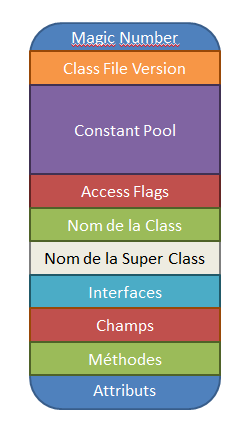
\includegraphics[scale=0.80]{JavaInternal.png}
        \caption{L'architecture de fichier .class \cite{ref_DexFormatvsJavabytecode}}
        \label{fig1}
    \end{figure}


    Les fichiers .class sont les fichiers exécutables par la machine virtuelle java. Chaque fichier .class contient les informations concernant une et une seule classe en Java. Dans ce fichier on trouve les instructions écrites en bytecode qui seront exécutées par la JVM. Nous présentons par la suite quelques détails, mais pour plus de détails il faut regarder les spécifications du java \cite{ref_specifications_java} .

    \subsubsection{Magic number}
    Il s'agit d'un attribut identifiant les fichiers d'execution Java \cite{ref_DexFormatvsJavabytecode}.

    \subsubsection{Class file version}
    Permet de déterminer la version minimum de la machine virtuelle de java qui pourra exécuter ce fichier. Donc si la version du fichier est supérieure à celle de la JVM, la machine virtuelle ne pourra pas l'exécuter.

    \subsubsection{Constant Pool}
    C'est une table qui contient toutes les constantes de la classe. Ces constantes peuvent être de types différents tels que \textbf{String},\textbf{Integer}, \textbf{Float}... etc. Par exemple, lorsque le fichier .java contient une variable qui a pour valeur 123456, cette table contiendra une case référencée par un indice et cette case stocke la valeur. De façon similaire, une chaîne de caractères telle que "ma belle chaîne de caractère" sera stockée dans une autre case dans la table.

    \subsubsection{Access Flags}
    Contient les informations sur l'accessibilité de la classe.

    \subsubsection{Class Name}
    On y trouve le nom de la classe.
    \subsubsection{Super Class Name}
    On y trouve le nom de la classe mère.

    \subsubsection{Interface}
    Si la classe implémente une interface, alors le nom de l'interface sera mentionné ici.

    \subsubsection{Champs}
    Les champs de la classe sont présentés ici avec leur niveau d'accessibilité private,protected ou public avec son nom et son type.

    \subsubsection{Methods}
    De façon similaire aux champs, chaque méthode est décrite par son niveau d'accessibilité, son nom, les types de ses paramètres et le type de retour.

    \subsection{Les types}
    Il existe deux sorts de type en java. Les types primitifs. L'autre sort est les types références. Une référence peut être de type classe ou de type tableau.
    \\

    On distingue ces types :
    \subsubsection{Les types numériques}
    Il existe deux catégories :
    \begin{itemize}
        \item Entier : tels que byte, short,int et char.
        \item A Virgule flottante : comme float et double.
    \end{itemize}

    \subsubsection{Le type boolean : } représente une valeur de vérité true ou false.
    \subsubsection{Le retour d'adresse : } le type returnAddress est un pointeur vers
    un des \textbf{Opcodes} de la JVM (utilisé par les instructions JSR, RET, et JSR$\_$W).

    \subsection{Les zones mémoires \cite{ref_zones_memeoire_java}}
    Il existe différentes zones de mémoire pour stocker les données pendant l'exécution d'un programme. Quelques zones sont crées au démarrage de la Java Virtual Machine et sont détruites quand elle s'arrête. Il existe d'autres zones qui sont crées lors de la création d'un nouveau thread, elles sont propores à ce thread et enfin détruites à la fin du thread.
    Nous allons détailler quelques zones :

    \subsubsection{Le registre program counter :} C'est un registre propre à chaque thread.

    \subsubsection{La pile d'exécution :} C'est une pile propre et privée à l'exécution de chaque thread. La pile est crée au moment de la création du thread et sera détruite à la fin du thread. Le rôle de la pile est de stocker les \textbf{Frames} que nous allons détailler dans la section suivante.

    \subsubsection{Le tas :} C'est une zone commune à tous les threads de la JVM. Il est créé au moment du démarrage de la JVM. Elle y stocke les données allouées dynamiquement telles que les instances des classes et les tableaux.

    \subsubsection{Zone de méthodes :}
    C'est une zone qui stocke le code de toutes les classes. Elle est partagée par tous les threads et elle stocke la \textbf{Constant Pool} \ref{Constant_Pool}, les champs et les variables de classe et des méthodes ainsi le code des méthodes.

    \subsubsection{Constant Pool : } \label{Constant_Pool} Pour chaque classe dans un fichier .class, il existe une table Constant Pool \ref{fig1}. Cette table est représentée dans une zone mémoire appelée Constant Pool. Elle contient toutes les constantes connues à la compilation et les références vers les méthodes qui doivent être résolues à l'exécution.

    \subsection{Les frames :}
    Une frame a pour rôle de stocker les données et les résultats partiels, on y stocke aussi la valeur de retour des appels aux méthodes. A chaque appel à une méthode, une nouvelle frame est crée. Elle sera détruite à la fin de l'appel. La freme est allouée dans la pile du thread qui l'a créé. Cette frame a son propre tableau de variables locales, sa pile d'opérandes et une référence vers la constant pool de la classe de la méthode appelée.

    \subsubsection{Les variables locales :}
    Chaque frame contient un tableau de variables locales. Une variable locale   simple en terme de taille peut contenir un type boolean, byte, char, short, int, float, reference, ou returnAddress. Pour stocker des variables locales de type double ou long, il faut la place de deux variables locales simples.
    Chaque variable est indexé par un indice. Comme dans une pile, l'indice de la première variable est 0. Les valeur des long ou double sont rangées dans deux cases consécutives.
    Lorsque une méthode statique est appelée, tous les paramètres sont passés dans des variables locales consécutives à partir de la variable locale d'adresse 0.
    Lorsque une méthode non statique est appelée, la référence sur l'objet à qui  est appelée a 0 pour indice de variable. Cette variable correspond à \textbf{this} en java. Les autres paramètres de la méthode seront rangés dans les cases qui suivent.

    \subsubsection{La pile des opérandes :} Chaque frame a une pile des opérandes. La JVM fournit des instructions pour charger des constantes ou des valeurs, depuis les variables locales dans la pile des opérandes. D'autres instructions récupèrent des opérandes de la pile des opérandes, réalisent une opération sur ces opérandes, puis stockent le résultat dans la pile d'opérandes de cette frame.

    \section{Conception}
    \subsection{Documentation de conception}
    \subsubsection{Structure globale}
    \subsubsection{Choix d'implémentation}
    \subsection{Algorithmes utilisés}

    \section{Validation}
    Dans le cadre de la validation de notre extension, nous avons utilisé la même batterie de tests que celle de notre compilateur decac. La différence est l'ajout de l'option -java lors de la compilation, ce qui permet de générer un fichier exécutable par la JVM.

    \subsection{Tests contextuels avec l'option -java}
    Nous avons créé un script de test pour la partie contextuelle qui est à peu de choses près le même que celui décrit dans la documentation de validation.
    \begin{flushleft}
        La différence concerne le fichier de test utilisé, puisqu'ici c'est ManualTestContextJava qui est lancé pour tous nos tests. En effet, nous ajoutons l'option -java au compilateur. Cela est utile pour tester la génération de fichier .class, et la possibilité d'utiliser du code java dans deca avec l'utilisation d'une methodJava.
    \end{flushleft}

    \subsubsection{Lancer les tests contextuels avec l'otpion -java}
    Pour lancer le script, il suffit de lancer le fichier \textbf{basic-context-java.sh} qui se trouve dans le répertoire \textit{gl28/src/test/script}. Ce script utilise notre large batterie de tests Oracle détaillée dans la documentation de validation.
    \begin{flushleft}
        Ces tests se trouvent dans le répertoire \textit{custom/option/java} des dossiers \textit{valid} et \textit{invalid} comme vous pouvez le voir ci-dessous.
    \end{flushleft}

    \subsubsection{Arborescence des tests contextuels}
    Le répertoire \textit{context} se trouve dans le dossier \textit{gl28/src/test/deca}.
    \begin{center}
        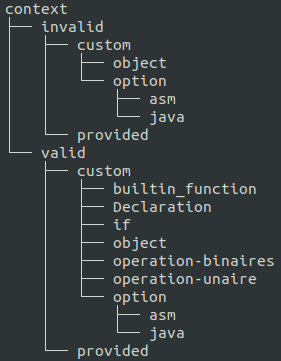
\includegraphics[scale=0.7]{treecontext.png}
    \end{center}


    \subsection{Tests de génération de code avec l'option -java}
    Enfin, concernant les tests de génération de code, nous avons décidé d'utiliser des tests de type "boîte noire". Pour chaque fichier de test nous créons un fichier .res avec la sortie attendue. Ainsi, pour chaque test, le script vérifie que le résultat obtenu en exécutant le fichier .class généré avec à notre compilateur correspond bien au résultat attendu.
    \begin{flushleft}
        Ces tests se trouvent dans le répertoire \textit{gl28/src/test/deca/codegen}, puis on distingue les tests valides et invalides.
    \end{flushleft}
    \subsubsection{Lancer les tests de génération de code}
    Le script qui permet de lancer l'exécution de tous les tests est \textbf{basic-gencode-java.sh}, il se trouve dans le répertoire \textit{gl28/src/test/script}.
    \begin{flushleft}Les tests sont donc lancés en utilisant l'option -java, ce qui permet de générer des fichiers .class exécutables par la JVM. La comparaison entre le résultat obtenu et le résultat attendu nous permet de nous assurer du bon fonctionnement de notre extension BYTE. Si le résultat n'est pas le bon, alors un message l'indique.
    \end{flushleft}

    \subsubsection{Arborescence des tests de génération de code}
    Le répertoire \textit{codegen} se trouve dans le dossier \textit{gl28/src/test/deca}. Le rôle de chacun de ces répertoires est expliqué dans la documentation de validation.
    \begin{center}
        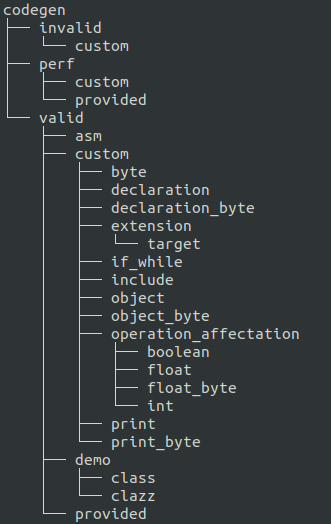
\includegraphics[scale=0.6]{treecodegen.png}
    \end{center}

    \subsubsection{Répertoire \textit{option/java}}
    En particulier, le répertoire \textit{extension} vérifie le bon fonctionnement de l'insertion de code java dans deca. Par exemple, il est possible d'importer une librairie java et de l'utiliser pour retourner un résultat.


    \section{Limitations}
    \subsection{Compatibilité Java-Deca}

    \newpage
    \printbibliography

\end{document}
